\documentclass[10pt,a4paper]{article}

\usepackage[utf8]{inputenc}
\usepackage[T1]{fontenc}
\usepackage[default]{lato}
\usepackage[margin=0pt]{geometry}
\usepackage{enumitem}
\usepackage{graphicx}
\usepackage{hyperref}
\usepackage{tabularx}
\usepackage{xcolor}
\usepackage{array}
\usepackage{microtype}
\usepackage{tikz}
\usepackage{fontawesome5}

\renewcommand{\familydefault}{\sfdefault}
\pagestyle{empty}
\setlength{\parindent}{0pt}
\setlength{\fboxsep}{0pt}
\setlength{\topskip}{0pt}
\raggedbottom
\graphicspath{{../assets/}{assets/}}
\hypersetup{colorlinks=true,urlcolor=accent,pdfauthor={Dinesh Gangatharan},pdftitle={Software Architect - Dinesh Gangatharan}}

\definecolor{bannerbg}{HTML}{20242C}
\definecolor{sidebarbg}{HTML}{EDEEF0}
\definecolor{accent}{HTML}{14919B}
\definecolor{heading}{HTML}{20242C}
\definecolor{muted}{HTML}{5B6168}

\newlength{\bannerheight}
\setlength{\bannerheight}{2.5cm}
\newlength{\sidepad}
\setlength{\sidepad}{14pt}

\newcommand{\sideheading}[1]{\vspace{0.9em}{\setlength{\fboxsep}{5pt}\colorbox{accent}{\parbox{\dimexpr\linewidth-10pt\relax}{\color{white}\bfseries\small #1}}}\par\vspace{0.5em}}
\newcommand{\mainheading}[1]{\vspace{0.3em}{\color{heading}\bfseries\Large #1}\par\vspace{0.15em}{\color{accent}\rule{\linewidth}{1.2pt}}\vspace{0.25em}}

\newcommand{\job}[5]{%
  \noindent{\bfseries #2}\hfill{\color{accent}\bfseries\small #1}\hspace{0.5em}\raisebox{-0.14cm}{\includegraphics[height=0.42cm,keepaspectratio]{#5}}\par
  {\color{muted}\itshape #3 --- \faMapMarker\ #4}\par\vspace{0.15em}}

\newcommand{\compactlist}{\begin{itemize}[leftmargin=1.1em,itemsep=0.12em,topsep=0.18em,parsep=0pt]}

\newcommand{\jobgap}{\vspace{0.55em}}

\newcommand{\prodrow}[3]{\noindent\begin{minipage}[t]{0.16\linewidth}\includegraphics[width=\linewidth]{#1}\end{minipage}\hfill\begin{minipage}[t]{0.80\linewidth}\href{#3}{#2}\end{minipage}\par\vspace{0.25em}}

\begin{document}
\noindent\colorbox{bannerbg}{%
  \parbox[t][\bannerheight][c]{\paperwidth}{%
    \hspace{0.9cm}\begin{minipage}[t]{\dimexpr\paperwidth-1.8cm\relax}
      {\fontsize{27}{30}\selectfont\bfseries\color{white} Dinesh Gangatharan}\par
      \vspace{0.15em}
      {\Large\color{accent} Senior Software Engineer / Software Architect}
    \end{minipage}%
  }%
}\par
\noindent
\begin{minipage}[t][\dimexpr\paperheight-\bannerheight\relax][t]{0.27\paperwidth}
  \colorbox{sidebarbg}{%
    \parbox[t][\dimexpr\paperheight-\bannerheight\relax][t]{\dimexpr\linewidth-2\sidepad\relax}{%
      \hspace{\sidepad}\begin{minipage}[t][\dimexpr\paperheight-\bannerheight\relax][t]{\dimexpr\linewidth-2\sidepad\relax}
      \setlength{\parskip}{0.25em}
      \vspace{0.6cm}
      \begin{center}
        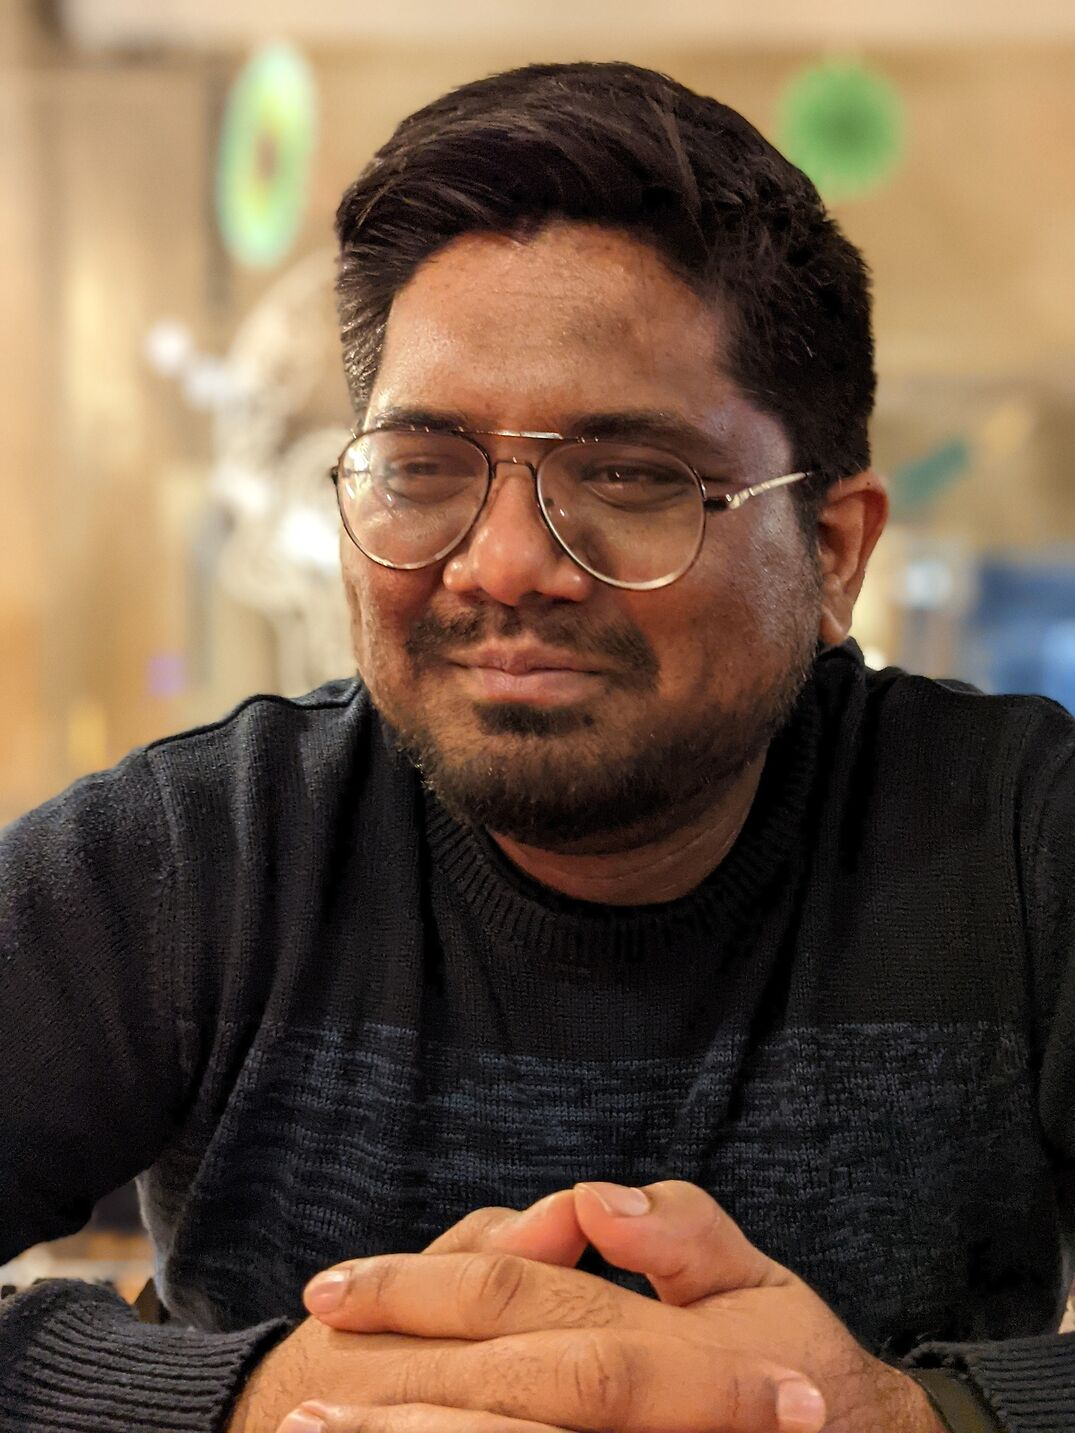
\includegraphics[width=3.4cm,keepaspectratio]{dinesh.jpeg}
      \end{center}
      \vfill
      \sideheading{SPECIALIST AREAS}
      \small Software Architecture\par
      Mobile Development\par
      Kotlin Multiplatform\par
      CI/CD \& Gradle\par
      Backend Integration

      \vfill
      \sideheading{CERTIFICATION}
      \noindent\begin{minipage}[t]{0.20\linewidth}
\includegraphics[width=\linewidth]{isaqb_badge.png}\end{minipage}\hfill\begin{minipage}[t]{0.76\linewidth}\hyphenpenalty=10000\exhyphenpenalty=10000\href{https://www.credly.com/badges/7d95218f-8be4-455a-950c-c17663d5b9e9}{\textbf{iSAQB -- CPSA-F}}\par\footnotesize Certified Professional, Software Architecture\end{minipage}

      \vfill
      \sideheading{PRODUCTS}
      \small
      \prodrow{erezept.png}{E-Rezept}{https://play.google.com/store/apps/details?id=de.gematik.ti.erp.app}
      \prodrow{barmer.png}{Barmer eCare}{https://play.google.com/store/apps/details?id=de.barmer.ecare}
      \prodrow{rewe.png}{REWE}{https://play.google.com/store/apps/details?id=de.rewe.app.mobile}
      \prodrow{authada.png}{AUTHADA}{https://play.google.com/store/apps/details?id=de.authada.id}

      \vfill
      \sideheading{CORE SKILLS}
      \small\raggedright
      \begin{itemize}[leftmargin=1.1em,itemsep=0.12em,topsep=0pt,parsep=0pt]
        \item Software Architecture
        \item Zero-Trust (ZETA)
        \item Kotlin Multiplatform (KMP)
        \item FHIR \& VZD
        \item CI/CD (Jenkins / Actions)
        \item Clean Architecture
      \end{itemize}

      \vfill
      \sideheading{LINKS}
      \footnotesize \mbox{\faGithub\ \href{https://github.com/dineshvg}{github.com/dineshvg}}\par
      \mbox{\faLinkedin\ \href{https://www.linkedin.com/in/dineshvg2310/}{linkedin.com/in/dineshvg2310}}

      \vfill
      \footnotesize \faEnvelope\ \href{mailto:dineshvg1023@gmail.com}{dineshvg1023@gmail.com}\par
      \faPhone\ +49 176 41637879\par
      \faMapMarker\ Stuttgart, Germany
      \vspace{0.6cm}
      \end{minipage}\hspace{\sidepad}%
  }
  }
\end{minipage}%
\begin{minipage}[t][\dimexpr\paperheight-\bannerheight\relax][t]{0.73\paperwidth}
  \hspace{0.75cm}\begin{minipage}[t][\dimexpr\paperheight-\bannerheight\relax][t]{\dimexpr\linewidth-1.5cm}
    \vspace{0.6cm}
    {\small\color{muted} Software architect and lead Android developer specialising in secure healthcare systems, Kotlin Multiplatform, scalable mobile architecture, and delivery automation.}

    \vspace{0.9em}
    \mainheading{Professional Experience}

    \job{Feb 2026--Present}{Gematik GmbH}{Software Architect}{Remote (Berlin)}{gematik-logo.png}
    \compactlist
      \item Lead Android Developer \& Architect for the E-Rezept Android app, serving 2M+ active users.
      \item Architected the Proof of Patient Presence (PoPP) mobile client ecosystem and Kotlin Multiplatform SDK, including Zero-Trust (ZETA) and NFC smartcard (PACE) integration.
      \item Engineered Push-Gateway integration for secure, end-to-end push notification routing and app ID validation across TI services.
      \item Designed App-to-App authentication and a local Mock IDP architecture with RFC 7636 PKCE for partner integration testing.
    \end{itemize}
    \jobgap

    \job{Sep 2023--Jan 2026}{Gematik GmbH}{Lead Developer}{Remote (Berlin)}{gematik-logo.png}
    \compactlist
      \item Responsible for the E-Rezept Android app and its connected FHIR-VZD backend services.
      \item Reimplemented FHIR parsing with Kotlinx Serialization and migrated the app to a multi-module architecture; built CI/CD infrastructure with reusable Gradle plugins.
      \item Led the team, mentored junior developers, and coordinated monthly releases; improved the app rating from 2.0 to 4.2.
    \end{itemize}
    \jobgap

    \job{Jan 2022--Aug 2023}{IBM iX DACH}{Senior Developer}{Remote (Berlin)}{ibm-logo.png}
    \compactlist
      \item Developed the digital maternity record feature and led a Flutter initiative to modernise time tracking, including a Python/Django backend.
      \item Collaborated with iOS engineers and used Kotlin Multiplatform and SwiftUI for cross-platform development.
    \end{itemize}
    \jobgap

    \job{Jul 2019--Dec 2021}{REWE Digital GmbH}{Software Engineer}{Cologne}{rewe-logo.png}
    \compactlist
      \item Delivered full-stack features with Android SDK, Kotlin, TypeScript, Node.js, REST, Firebase, and automated testing.
      \item Designed and improved scalable architectures using MVVM, MVP, and MVI patterns.
    \end{itemize}
    \jobgap

    \job{Nov 2016--Jun 2019}{AUTHADA GmbH}{Software Engineer}{Darmstadt}{authada-logo.jpg}
    \compactlist
      \item Developed certification functionality for the Android application.
      \item Migrated Java code to Kotlin using Clean Code principles and MVP.
    \end{itemize}

    \begin{minipage}[t]{0.48\linewidth}
      \mainheading{Education}
      \noindent\begin{minipage}[t]{0.76\linewidth}
        \raggedright{\bfseries M.Sc. Electrical Engineering and IT}\par
        {\small TU Darmstadt \hfill 2014--2017}
      \end{minipage}\hfill\raisebox{-0.3cm}{
\includegraphics[height=0.8cm,keepaspectratio]{tud.png}}\par\vspace{0.35em}
      \noindent\begin{minipage}[t]{0.76\linewidth}
        \raggedright{\bfseries B.E. Electrical Engineering}\par
        {\small Anna University \hfill 2006--2010}
      \end{minipage}\hfill\raisebox{-0.3cm}{
\includegraphics[height=0.8cm,keepaspectratio]{anna_univ_logo.png}}
    \end{minipage}\hfill
    \begin{minipage}[t]{0.48\linewidth}
      \mainheading{Publications}
      \footnotesize
      \begin{itemize}[leftmargin=1.1em,itemsep=0.3em,topsep=0pt,parsep=0pt]
        \item \href{https://www.researchgate.net/publication/320165052_Exercise_Monitoring_On_Consumer_Smart_Phones_Using_Ultrasonic_Sensing}{Exercise Monitoring on Consumer Smartphones Using Ultrasonic Sensing} (2017)
        \item \href{https://www.researchgate.net/publication/324942766_Fitness_Activity_Recognition_on_Smartphones_Using_Doppler_Measurements}{Fitness Activity Recognition on Smartphones Using Doppler Measurements} (2018)
      \end{itemize}
    \end{minipage}

    \vfill
    {\color{accent}\rule{\linewidth}{0.8pt}}\par\vspace{0.4em}
    {\centering\small\color{muted} \href{https://dineshvg.github.io}{dineshvg.github.io}\par}
    \vspace{0.5cm}
  \end{minipage}\hspace{0.75cm}
\end{minipage}
\end{document}
